\de{ĐỀ THI HỌC KỲ I NĂM HỌC 2022-2023}{THPT Nguyễn An Ninh}


\begin{bt}%[0T2Y1-2]%[Dự án đề kiểm tra HKI NH22-23-Mui Doan]%[THPT Nguyễn An Ninh-Sở Hồ Chí Minh]
	Cho $4$ cặp số $(-1;-3)$,$(1;2)$, $(-2;0)$, $(4;-1)$ và cho bất phương trình 
	\[2 x-3 y+4 \leq 0.\quad (1)\]
	Hãy liệt kê những cặp số là nghiệm của bất phương trình $(1)$ và những cặp số \textbf{không} là nghiệm của bất phương trình $(1)$.
	\loigiai{
		\begin{itemize}
			\item $(1;2)$, $(-2;0)$  là nghiệm của bất phương trình $(1)$.
			\item $(-1;-3)$, $(4;-1)$ \textbf{không} là nghiệm của bất phương trình $(1)$.
		\end{itemize}
	}
\end{bt} 

\begin{bt}%[0T3Y1-2]%[Dự án đề kiểm tra HKI NH22-23-Mui Doan]%[THPT Nguyễn An Ninh-Sở Hồ Chí Minh]
	\immini{
		Cho hàm số $y=f(x)$ có đồ thị như hình vẽ bên dưới
		\begin{listEX}
			\item Tìm tập xác định và tập giá trị của hàm số.
			\item Tính $f(-1)$, $f(6)$.
		\end{listEX}
	}{
		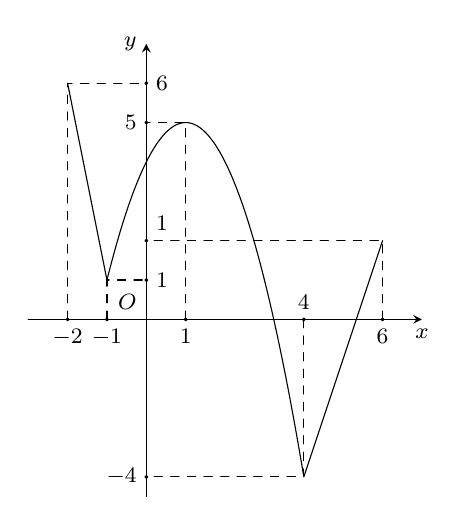
\begin{tikzpicture}[scale=0.5,>=stealth, font=\footnotesize, line join=round, line cap=round]
			\def\a{-1} \def\b{2} \def\c{4} % Hệ số
			\def\xmin{-3} \def\xmax{7}
			\def\ymin{-4.5} \def\ymax{7} 
			%	\draw[color=gray!50,dashed] (\xmin,\ymin) grid (\xmax,\ymax); 
			\draw[->] (\xmin,0)--(\xmax,0) node [below]{$x$};
			\draw[->] (0,\ymin)--(0,\ymax) node [left]{$y$};
			\node at (0,0) [above left]{$O$};
			\clip (\xmin+0.1,\ymin+0.1) rectangle (\xmax-0.5,\ymax-0.1);
			\draw[smooth,samples=300,domain=-1:4] plot(\x,{\a*(\x)^2+\b*(\x)+\c});
			\draw[dashed] (-2,0)|-(0,6) (-1,0)|-(0,1) (1,0)|-(0,5) (4,0)|-(0,-4) (6,0)|-(0,2);
			\draw (-2,6)--(-1,1) (4,-4)--(6,2);
			\draw[fill=black]
			(-2,0)node[below]{$-2$}circle(1pt)
			(-1,0)node[below]{$-1$}circle(1pt)
			(1,0)node[below]{$1$}circle(1pt)
			(6,0)node[below]{$6$}circle(1pt)
			(4,0)node[above]{$4$}circle(1pt)
			(0,6)node[right]{$6$}circle(1pt)
			(0,5)node[left]{$5$}circle(1pt)
			(0,-4)node[left]{$-4$}circle(1pt)
			(0,1)node[right]{$1$}circle(1pt)
			(0,2)node[above right]{$1$}circle(1pt);
		\end{tikzpicture}
	}
	\loigiai{
		\begin{listEX}
			\item Tập xác định $\mathscr{D}=[-2;6]$; tập giá trị $I=[-4;6]$.
			\item $f(-1)=1$, $f(6)=2$.
		\end{listEX}
	}
\end{bt} 

\begin{bt}%[0T3B1-3]%[Dự án đề kiểm tra HKI NH22-23-Mui Doan]%[THPT Nguyễn An Ninh-Sở Hồ Chí Minh]
	Cho hàm số $y=-3 x^2-4 x+\dfrac{5}{3}$ có đồ thị là parabol $(P)$.
	\begin{listEX}
		\item Tìm tọa độ đỉnh $S$ và trục đối xứng của parabol $(P)$.
		\item Tìm tọa độ giao điểm của đồ thị $(P)$ với trục hoành.
	\end{listEX}
	\loigiai{
			\begin{listEX}
			\item Ta có $a=-3$; $b=-4$; $c=\dfrac{5}{3}$; \\
			$x=-\dfrac{b}{2a}= -\dfrac{2}{3}\Rightarrow y=-3\cdot \left(-\dfrac{2}{3}\right)^2-4\left(-\dfrac{2}{3}\right)+\dfrac{5}{3}=-\dfrac{2}{3}$.\\
			Đỉnh $S\left(-\dfrac{2}{3} ; 3\right)$ và trục đối xứng $x=-\dfrac{2}{3}$;
			\item Phương trình hoành độ giao điểm của $(P)$ và trục hoành
			$$-3 x^2-4 x+\dfrac{5}{3}=0\Leftrightarrow\hoac{&x=\dfrac{1}{3}\\&x=-\dfrac{5}{3}.}$$
			Vậy độ giao điểm của đồ thị $(P)$ với trục hoành là
			$A\left(\dfrac{1}{3} ; 0\right)$ và $B\left(-\dfrac{5}{3} ; 0\right)$.
		\end{listEX}
	}
\end{bt} 

\begin{bt}%[0T5B2-2]%[Dự án đề kiểm tra HKI NH22-23-Mui Doan]%[THPT Nguyễn An Ninh-Sở Hồ Chí Minh]
	Cho hình bình hành $ABCD$ tâm $O$. Rút gọn  
	$\vec{a}=\overrightarrow{O A}+\overrightarrow{B O}-\overrightarrow{C D}$.
	\loigiai{
		\immini{
	Ta có 	
	\allowdisplaybreaks
	\begin{eqnarray*}
		\vec{a}&=&\overrightarrow{O A}+\overrightarrow{B O}-\overrightarrow{C D}
		\\
		&=&\overrightarrow{B O}+\overrightarrow{O A}-\overrightarrow{C D}
		\\
		&=&\overrightarrow{B A}+\overrightarrow{DC}
		\\
		&=&\overrightarrow{B A}+\overrightarrow{AB}
		\\
		&=&\overrightarrow{0}.
	\end{eqnarray*}
	}
	{
	\begin{tikzpicture}
		\path (0,0) coordinate (A)
		(2,0) coordinate (B)
		 ($ (B)!1!-90:(A)$) coordinate (C)
		 ($(A)!1!90:(B)$) coordinate (D)
		 ($(A)!.5!(C)$)  coordinate (O)
		 ;
	\draw (B)--(C)--(D)--(A)--cycle (A)--(C) (B)--(D);
	\foreach \t/\g in {A/180,B/0,C/0,D/180,O/0}{
		\draw[fill=black] (\t) circle (1pt) node[shift={(\g:7pt)},font=\scriptsize]{$ \t $};
	}
	\end{tikzpicture}
		}
	}
\end{bt} 

\begin{bt}%[0T5K2-2]%[Dự án đề kiểm tra HKI NH22-23-Mui Doan]%[THPT Nguyễn An Ninh-Sở Hồ Chí Minh]
	Cho tam giác $A B C$. Điểm $I$ trên cạnh $A C$ sao cho $C I=\dfrac{1}{4} C A$. Phân tích $\overrightarrow{B I}$ theo $2$ véc-tơ $\overrightarrow{A B}$ và $\overrightarrow{AC}$.
	%\dapso{$\overrightarrow{B I}=\dfrac{3}{4} \overrightarrow{A C}-\overrightarrow{A B}$.}
	\loigiai{
	\immini{
	Vì $I$ trên cạnh $A C$ và $C I=\dfrac{1}{4} CA$ nên 
	\allowdisplaybreaks
	\begin{eqnarray*}
		&&\overrightarrow{CI}=\dfrac{1}{4} \overrightarrow{ CA}
		\\
		&\Leftrightarrow&\overrightarrow{CB}+\overrightarrow{BI}=\dfrac{1}{4} \overrightarrow{ CA}
		\\
		&\Leftrightarrow&\overrightarrow{CA}+\overrightarrow{AB}+\overrightarrow{BI}=\dfrac{1}{4} \overrightarrow{ CA}
		\\
		&\Leftrightarrow&\overrightarrow{BI}=-\dfrac{3}{4} \overrightarrow{ CA}-\overrightarrow{AB}
		\\
		&\Leftrightarrow&\overrightarrow{BI}=-\overrightarrow{AB}+\dfrac{3}{4} \overrightarrow{AC}.
	\end{eqnarray*}
		}
	{
	\begin{tikzpicture}
	\path (0,0) coordinate (A)++
	(-2,-3) coordinate (B)
	(3,-3) coordinate (C)
	($(C)!1/4!(A)$) coordinate (I)
	;
	\draw (A)--(B)--(C)--cycle (B)--(I);
	\foreach \t/\g in {A/90,B/180,C/0,I/0}{
		\draw[fill=black] (\t) circle (1pt) node[shift={(\g:7pt)},font=\scriptsize]{$ \t $};
	}
	\end{tikzpicture}
		}
	}
\end{bt} 


\begin{bt}%[0T3Y1-2]%[Dự án đề kiểm tra HKI NH22-23- Nguyễn Văn Sang]%[THPT Nguyễn An Ninh]
Tìm tập xác định của hàm số $f(x)=\sqrt{5-3 x}$.
%\dapso{$\mathscr{D}=\left(-\infty;\dfrac{5}{3}\right]$.}
\loigiai{
Hàm số có nghĩa khi $5-3 x\geq 0\Leftrightarrow x\leq \dfrac{5}{3}.$\\
Vậy tập xác định $\mathscr{D}=\left(-\infty;\dfrac{5}{3}\right]$.
}
\end{bt} 

\begin{bt}%[0T3B2-2]%[Dự án đề kiểm tra HKI NH22-23- Nguyễn Văn Sang]%[THPT Nguyễn An Ninh]
Cho hàm số bậc hai $y=f(x)=a x^2+b x+c$ có $f(2)=11$, $f(-5)=144$ và đồ thị của hàm số đi qua điểm $A(0 ;-1)$. Xác định giá trị của các hệ số $a$, $b$, $c$.
%\dapso{$a=5$, $b=-4$,$c=-1$.}
\loigiai{
	Ta có $f(x)=a x^2+b x+c$, từ $f(2)=11$, $f(-5)=144$ và đồ thị của hàm số đi qua điểm $A(0 ;-1)$ ta được hệ phương trình
	$$\heva{& 4a+2b+c=11\\ & 25a-5b+c=144 \\ & 0a+0b+c=-1}\Leftrightarrow \heva{& a=5 \\ & b=-4\\&c=-1.} $$
	Vậy $a=5$, $b=-4$,$c=-1$.
}
\end{bt} 

\begin{bt}%[0T5B4-1]%[Dự án đề kiểm tra HKI NH22-23- Nguyễn Văn Sang]%[THPT Nguyễn An Ninh]
Cho tam giác $ABC$ vuông tại $A$ có $AC=2022 a$. Tính $\overrightarrow{AC} \cdot \overrightarrow{CB}$ theo $a$.
%\dapso{$\overrightarrow{AC} \cdot \overrightarrow{C B}=-2022^2a^2$.}
\loigiai{
\immini
{
Vì tam giác $ABC$ vuông tại $A$ nên $\overrightarrow{AB}\cdot\overrightarrow{AC}=0$.\\
Ta có 
\begin{eqnarray*}
	\overrightarrow{AC} \cdot \overrightarrow{CB}&=&\overrightarrow{AC} \cdot\left( \overrightarrow{AB}-\overrightarrow{AC}\right)\\
	&=&\overrightarrow{AC} \cdot \overrightarrow{AB}-\overrightarrow{AC}\cdot \overrightarrow{AC}\\
	&=&0-AC^2=-2022^2a^2.
\end{eqnarray*}
}
{
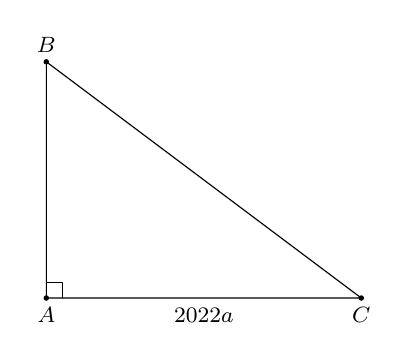
\begin{tikzpicture}[>=stealth,line join=round,line cap=round,font=\footnotesize,scale=1]
	\fill (0,0)  coordinate (A) circle (1pt) node[below]{$A$};
	\fill (0,3) coordinate (B) circle (1pt) node[above]{$B$};
	\fill (4,0) coordinate (C) circle (1pt) node[below]{$C$};
	\draw (A)--(C)node[midway, below]{$2022a$}--(B)--cycle ;
	\draw (A)--++(90:0.2)--++(0:0.2)--++(-90:0.2);
\end{tikzpicture}
}
}
\end{bt} 

\begin{bt}%[0T4K3-1]%[Dự án đề kiểm tra HKI NH22-23- Nguyễn Văn Sang]%[THPT Nguyễn An Ninh]
\immini{
Từ vị trí $A$ người ta quan sát một cây cao (hình vẽ). Biết $AH=4\,\mathrm{m}$, $HB=20\, \mathrm{m}$, $\widehat{BAC}=45^{\circ}$. Chiều cao của cây bằng bao nhiêu? (Độ dài cạnh lấy tròn đến phần nguyên, góc lấy tròn đến phút).
}{
\tikzset{
	ex_markstyle/.style={},
	ex_mark/.style  n args={1}{decoration={ markings, %
			mark= at position 0.5 with
			with{
				\ifnum#1=1
				\draw[ex_markstyle] (0pt,-2pt) -- (0pt,2pt);
				\fi
				\ifnum#1=2
				\draw[ex_markstyle] (-1pt,-2pt) -- (-1pt,2pt);
				\draw[ex_markstyle] (1pt,-2pt) -- (1pt,2pt);
				\fi
				\ifnum#1=3
				\draw[ex_markstyle] (-2pt,-2pt) -- (-2pt,2pt);
				\draw[ex_markstyle] (0pt,-2pt) -- (0pt,2pt);
				\draw[ex_markstyle] (2pt,-2pt) -- (2pt,2pt);
				\fi
				\ifnum#1=4
				\draw[ex_markstyle] (-1pt,-1pt) -- (1pt,1pt);
				\draw[ex_markstyle] (-1pt,1pt) -- (1pt,-1pt);
				\fi
		}},
		pic actions/.append code=\tikzset{postaction=decorate}},
}
%------
\definecolor{lightcornflowerblue}{rgb}{0.6, 0.81, 0.93}
\definecolor{cadmiumgreen}{rgb}{0.0, 0.42, 0.24}
\definecolor{trueblue}{rgb}{0.0, 0.45, 0.81}
\definecolor{tumbleweed}{rgb}{0.87, 0.67, 0.53}%màu cát
\definecolor{forestgreen(web)}{rgb}{0.13, 0.55, 0.13}
\definecolor{darkpastelgreen}{rgb}{0.01, 0.75, 0.24}
\definecolor{bronze}{rgb}{0.8, 0.5, 0.2}

\begin{tikzpicture}[line join=round, line cap=round,scale=1,transform shape]
\clip (-2.5,-2.5) rectangle (3,2.5);
\tikzset{cay/.pic={
\def\T{ %Thân
(-.33,0)%trái
..controls +(-50:.25) and +(40:.45) ..  (-.57,-1.45)
..controls +(20:.1) and +(-160:.15) ..  (-.1,-1.3)
..controls +(-120:.1) and +(60:.15) ..  (-.2,-1.6)
..controls +(-30:.1) and +(-140:.15) ..  (.15,-1.3)
..controls +(-20:.1) and +(-160:.15) ..  (.57,-1.4)
..controls +(170:.4) and +(-160:.1) ..  (.35,0)
..controls +(110:.5) and +(80:.5) ..  (-.33,0)
;}
%\draw \T;
\fill[bronze] \T;
\def\C{ 
(0,.3)
..controls +(-100:.25) and +(-60:.2) ..  (-.3,.1)
..controls +(-100:.25) and +(-60:.2) ..  (-.6,0)
..controls +(-120:.45) and +(-110:.35) ..  (-1,.2)
..controls +(-150:.5) and +(-140:.35) ..  (-1.15,.7)%nút giao
..controls +(-170:.4) and +(-170:.35) ..  (-1,1.15)
..controls +(140:.35) and +(110:.4) ..  (-.37,1.35)
..controls +(110:.25) and +(80:.3) ..  (-.15,1.35)
..controls +(80:.3) and +(95:.8) ..  (.55,1.1)
..controls +(80:.2) and +(95:.2) ..  (.8,1.1)
..controls +(20:.1) and +(95:.1) ..  (.95,1)
..controls +(-20:.4) and +(35:.25) ..  (1,.47)
..controls +(-30:.3) and +(-20:.3) ..  (.75,0.05)%nút giao
..controls +(-120:.3) and +(-60:.2) ..  (.35,0)
..controls +(175:.2) and +(-160:.1) ..  (.2,0.2)
..controls +(-160:.1) and +(-70:.1) ..  (0,.3)
;}
\draw \C;
\fill[forestgreen(web)] \C;
\def\C1{ 
(-1.15,.7)%nút giao
..controls +(-170:.4) and +(-170:.35) ..  (-1,1.15)
..controls +(140:.35) and +(110:.4) ..  (-.37,1.35)
..controls +(110:.25) and +(80:.3) ..  (-.15,1.35)
..controls +(80:.3) and +(95:.8) ..  (.55,1.1)
..controls +(80:.2) and +(95:.2) ..  (.8,1.1)
..controls +(20:.1) and +(95:.1) ..  (.95,1)
..controls +(-20:.4) and +(35:.25) ..  (1,.47)
..controls +(-50:.5) and +(-85:.6) ..  (.65,.55)% gần nút giao
..controls +(-160:.4) and +(-120:.4) ..  (0,.7)
..controls +(-150:.2) and +(-80:.4) ..  (-.63,.6)
..controls +(-140:.5) and +(-130:.4) ..  (-1.15,.7)
;}
%\draw \C1;
\fill[darkpastelgreen] \C1;
\def\G{ %Gân
(-.8,.2)
..controls +(-35:.1) and +(130:.35) ..  
(-.32,0)%nút giao
..controls +(-40:.1) and +(45:.35) ..  (-.42,-1.25)
(-.32,0)%nút giao
..controls +(120:.1) and +(-45:.35) ..  (-.58,.45)
(-.32,0)%nút giao
..controls +(80:.1) and +(-170:.35) ..  (-.05,.45)
(-.28,.3)
..controls +(80:.1) and +(-60:.05) ..  (-.35,.55)
%Gân phải
(.45,-1.3)
..controls +(130:.6) and +(-160:.3) ..  (.6,0.35)
(.37,0)
..controls +(35:.2) and +(-150:.1) ..  (.66,0.15)
(.37,0)
..controls +(80:.2) and +(-40:.1) ..  (.18,0.4)
(.31,0.25)
..controls +(80:.1) and +(-150:.1) ..  (.38,0.5)
(.25,-0.15)
..controls +(-110:.05) and +(110:.05) ..  (.2,-0.5)%gân dọc
(.2,-0.25)
..controls +(-110:.05) and +(110:.05) ..  (.17,-0.45)
(-.2,-0.15)
..controls +(-70:.1) and +(110:.05) ..  (-.18,-0.5)
(-.15,-0.15)
..controls +(-70:.1) and +(110:.05) ..  (-.15,-0.7)
(-.05,-0.8)
..controls +(-80:.15) and +(-10:.15) ..  (-.3,-1.28)
(-.1,-0.9)
..controls +(-110:.1) and +(20:.05) ..  (-.2,-1.1)
(.1,-1)
..controls +(-50:.05) and +(120:.05) ..  (.15,-1.2)
(.1,-1.15)
..controls +(-50:.05) and +(120:.05) ..  (.12,-1.2)
(.15,-.75)
..controls +(-120:.1) and +(-140:.1) ..  (.22,-.9)
..controls +(70:.12) and +(120:.05) ..  (.18,-.9)
;}

\draw \G;

}}

\path
(2,0)pic[scale=.8]{cay}
;
\path 	(2,-1.1) coordinate (B)
		(-2,-1.1) coordinate (H)
		(-2,-.5) coordinate (A)
		(2,1.25) coordinate (C)
		;
		\node at (B) [below]{\tiny $B$};
		\node at (H) [below]{\tiny $H$};
		\node at (A) [left]{\tiny $A$};
		\node at (C) [above]{\tiny $C$};
		\node at (-2,-.8) [left]{\tiny $4$};
		\node at (0,-1.1) [below]{\tiny $20$};
\draw (B)--(H)--(A)--(C) (A)--(B);
\draw    pic["\tiny $45^\circ$", draw=black, angle eccentricity=1.8, ex_mark=1,angle radius=.4cm, color=blue]
					{angle=B--A--C};
\draw    pic[draw=black, angle radius=.1cm]
	{right angle=A--H--B}; 
\end{tikzpicture}
}
%\dapso{$17\,\mathrm{m}$.}
\loigiai{
	\immini
	{
	Xét tam giác $ABH$ vuông tại $H$ ta có
	\begin{itemize}
		\item $AB=\sqrt{AH^2+BH^2}=\sqrt{416}$.
		\item $\cos \widehat{HAB}=\dfrac{AH}{AB}=\dfrac{4}{\sqrt{416}}\Rightarrow \widehat{HAB}\approx 78^\circ41'$.
	\end{itemize}
	Xét tứ giác $ACBH$ ta được $$\widehat{ACB}=360^\circ-90^\circ90^\circ-(78^\circ41'+45^\circ)\approx 56^\circ19'.$$
	}
	{
	
	\tikzset{
		ex_markstyle/.style={},
		ex_mark/.style  n args={1}{decoration={ markings, %
				mark= at position 0.5 with
				with{
					\ifnum#1=1
					\draw[ex_markstyle] (0pt,-2pt) -- (0pt,2pt);
					\fi
					\ifnum#1=2
					\draw[ex_markstyle] (-1pt,-2pt) -- (-1pt,2pt);
					\draw[ex_markstyle] (1pt,-2pt) -- (1pt,2pt);
					\fi
					\ifnum#1=3
					\draw[ex_markstyle] (-2pt,-2pt) -- (-2pt,2pt);
					\draw[ex_markstyle] (0pt,-2pt) -- (0pt,2pt);
					\draw[ex_markstyle] (2pt,-2pt) -- (2pt,2pt);
					\fi
					\ifnum#1=4
					\draw[ex_markstyle] (-1pt,-1pt) -- (1pt,1pt);
					\draw[ex_markstyle] (-1pt,1pt) -- (1pt,-1pt);
					\fi
			}},
			pic actions/.append code=\tikzset{postaction=decorate}},
	}
	%------
	\definecolor{lightcornflowerblue}{rgb}{0.6, 0.81, 0.93}
	\definecolor{cadmiumgreen}{rgb}{0.0, 0.42, 0.24}
	\definecolor{trueblue}{rgb}{0.0, 0.45, 0.81}
	\definecolor{tumbleweed}{rgb}{0.87, 0.67, 0.53}%màu cát
	\definecolor{forestgreen(web)}{rgb}{0.13, 0.55, 0.13}
	\definecolor{darkpastelgreen}{rgb}{0.01, 0.75, 0.24}
	\definecolor{bronze}{rgb}{0.8, 0.5, 0.2}
	
	\begin{tikzpicture}[line join=round, line cap=round,scale=1,transform shape]
		\clip (-2.5,-2.5) rectangle (3,2.5);
		\tikzset{cay/.pic={
				\def\T{ %Thân
					(-.33,0)%trái
					..controls +(-50:.25) and +(40:.45) ..  (-.57,-1.45)
					..controls +(20:.1) and +(-160:.15) ..  (-.1,-1.3)
					..controls +(-120:.1) and +(60:.15) ..  (-.2,-1.6)
					..controls +(-30:.1) and +(-140:.15) ..  (.15,-1.3)
					..controls +(-20:.1) and +(-160:.15) ..  (.57,-1.4)
					..controls +(170:.4) and +(-160:.1) ..  (.35,0)
					..controls +(110:.5) and +(80:.5) ..  (-.33,0)
					;}
				%\draw \T;
				\fill[bronze] \T;
				\def\C{ 
					(0,.3)
					..controls +(-100:.25) and +(-60:.2) ..  (-.3,.1)
					..controls +(-100:.25) and +(-60:.2) ..  (-.6,0)
					..controls +(-120:.45) and +(-110:.35) ..  (-1,.2)
					..controls +(-150:.5) and +(-140:.35) ..  (-1.15,.7)%nút giao
					..controls +(-170:.4) and +(-170:.35) ..  (-1,1.15)
					..controls +(140:.35) and +(110:.4) ..  (-.37,1.35)
					..controls +(110:.25) and +(80:.3) ..  (-.15,1.35)
					..controls +(80:.3) and +(95:.8) ..  (.55,1.1)
					..controls +(80:.2) and +(95:.2) ..  (.8,1.1)
					..controls +(20:.1) and +(95:.1) ..  (.95,1)
					..controls +(-20:.4) and +(35:.25) ..  (1,.47)
					..controls +(-30:.3) and +(-20:.3) ..  (.75,0.05)%nút giao
					..controls +(-120:.3) and +(-60:.2) ..  (.35,0)
					..controls +(175:.2) and +(-160:.1) ..  (.2,0.2)
					..controls +(-160:.1) and +(-70:.1) ..  (0,.3)
					;}
				\draw \C;
				\fill[forestgreen(web)] \C;
				\def\C1{ 
					(-1.15,.7)%nút giao
					..controls +(-170:.4) and +(-170:.35) ..  (-1,1.15)
					..controls +(140:.35) and +(110:.4) ..  (-.37,1.35)
					..controls +(110:.25) and +(80:.3) ..  (-.15,1.35)
					..controls +(80:.3) and +(95:.8) ..  (.55,1.1)
					..controls +(80:.2) and +(95:.2) ..  (.8,1.1)
					..controls +(20:.1) and +(95:.1) ..  (.95,1)
					..controls +(-20:.4) and +(35:.25) ..  (1,.47)
					..controls +(-50:.5) and +(-85:.6) ..  (.65,.55)% gần nút giao
					..controls +(-160:.4) and +(-120:.4) ..  (0,.7)
					..controls +(-150:.2) and +(-80:.4) ..  (-.63,.6)
					..controls +(-140:.5) and +(-130:.4) ..  (-1.15,.7)
					;}
				%\draw \C1;
				\fill[darkpastelgreen] \C1;
				\def\G{ %Gân
					(-.8,.2)
					..controls +(-35:.1) and +(130:.35) ..  
					(-.32,0)%nút giao
					..controls +(-40:.1) and +(45:.35) ..  (-.42,-1.25)
					(-.32,0)%nút giao
					..controls +(120:.1) and +(-45:.35) ..  (-.58,.45)
					(-.32,0)%nút giao
					..controls +(80:.1) and +(-170:.35) ..  (-.05,.45)
					(-.28,.3)
					..controls +(80:.1) and +(-60:.05) ..  (-.35,.55)
					%Gân phải
					(.45,-1.3)
					..controls +(130:.6) and +(-160:.3) ..  (.6,0.35)
					(.37,0)
					..controls +(35:.2) and +(-150:.1) ..  (.66,0.15)
					(.37,0)
					..controls +(80:.2) and +(-40:.1) ..  (.18,0.4)
					(.31,0.25)
					..controls +(80:.1) and +(-150:.1) ..  (.38,0.5)
					(.25,-0.15)
					..controls +(-110:.05) and +(110:.05) ..  (.2,-0.5)%gân dọc
					(.2,-0.25)
					..controls +(-110:.05) and +(110:.05) ..  (.17,-0.45)
					(-.2,-0.15)
					..controls +(-70:.1) and +(110:.05) ..  (-.18,-0.5)
					(-.15,-0.15)
					..controls +(-70:.1) and +(110:.05) ..  (-.15,-0.7)
					(-.05,-0.8)
					..controls +(-80:.15) and +(-10:.15) ..  (-.3,-1.28)
					(-.1,-0.9)
					..controls +(-110:.1) and +(20:.05) ..  (-.2,-1.1)
					(.1,-1)
					..controls +(-50:.05) and +(120:.05) ..  (.15,-1.2)
					(.1,-1.15)
					..controls +(-50:.05) and +(120:.05) ..  (.12,-1.2)
					(.15,-.75)
					..controls +(-120:.1) and +(-140:.1) ..  (.22,-.9)
					..controls +(70:.12) and +(120:.05) ..  (.18,-.9)
					;}
				
				\draw \G;
				
		}}
		
		\path
		(2,0)pic[scale=.8]{cay}
		;
		\path 	(2,-1.1) coordinate (B)
		(-2,-1.1) coordinate (H)
		(-2,-.5) coordinate (A)
		(2,1.25) coordinate (C)
		;
		\node at (B) [below]{\tiny $B$};
		\node at (H) [below]{\tiny $H$};
		\node at (A) [left]{\tiny $A$};
		\node at (C) [above]{\tiny $C$};
		\node at (-2,-.8) [left]{\tiny $4$};
		\node at (0,-1.1) [below]{\tiny $20$};
		\draw (B)--(H)--(A)--(C) (A)--(B)--(C);
		\draw    pic["\tiny $45^\circ$", draw=black, angle eccentricity=1.8, ex_mark=1,angle radius=.4cm, color=blue]
		{angle=B--A--C};
		\draw    pic[draw=black, angle radius=.1cm]
		{right angle=A--H--B};
	\end{tikzpicture}
	}\noindent
	Áp dụng định lý sin trong tam giác $ABC$ ta có
$$\dfrac{BC}{\sin A}=\dfrac{AB}{\sin C}\Leftrightarrow BC=\dfrac{AB\cdot \sin A}{\sin C}\approx17{,}396.$$
Làm tròn đến phần nguyên (hàng đơn vị) ta được $BC=17$ m.\\
Vậy chiều cao của cây là $17$ m.
}
\end{bt} 

\begin{bt}%[0T2G2-2]%[Dự án đề kiểm tra HKI NH22-23- Nguyễn Văn Sang]%[THPT Nguyễn An Ninh]
Trong một cuộc thi gói bánh vào dịp năm mới, mỗi đội chơi được sử dụng tối đa $20\,\mathrm{kg}$ gạo nếp, $2\,\mathrm{kg}$ thị ba chỉ, $5\,\mathrm{kg}$ đậu xanh để gói bánh chưng và bánh tét. Để gói một cái bánh chưng cần $0{,}4\,\mathrm{kg}$ gạo nếp, $0{,}05\,\mathrm{kg}$ thịt và $0{,}1\,\mathrm{kg}$ đậu xanh; để gói một cái bánh tét cần $0{,}6\,\mathrm{kg}$ gạo nếp, $0{,}075\,\mathrm{kg}$ thịt và $0{,}15\,\mathrm{kg}$ đậu xanh. Mỗi cái bánh chưng nhận được $5$ điểm thưởng, mỗi cái bánh tét nhận được $7$ điểm thưởng. Hỏi điểm thưởng cao nhất có thể đạt được là bao nhiêu?
%\dapso{$200$ điểm.}
\loigiai{
Gọi $x$, $y$ lần lượt là số bánh chưng và bánh tét gói được $\left(x, y \in \mathbb{N}^*\right)$.\\
Số điểm thưởng đạt được là  $5x+7y$ (điểm).\\
Theo bài ra ta có hệ bất phương trình $$\heva{&0,4x+0,6y \leq 20 \\& 0,05x+0,075y \leq 2 \\& 0,1x+0,15y \leq 5 \\& x \geq 0 \\& y \geq 0} \Leftrightarrow \heva{&2x+3y \leq 100 \\& 2x+3y \leq 80 \\& 2x+3y \leq 100 \\& x \geq 0 \\& y \geq 0} \Leftrightarrow \heva{&2x+3y \leq 80 \\& x \geq 0 \\& y \geq 0.} (I)$$
\immini
{
Yêu cầu bài toán trở thành tìm $(x;y)$ thỏa mãn hệ $(I)$ để $F(x;y)=5x+7y$ đạt giá trị lớn nhất.\\
Vẽ và xác định miền nghiệm của $(I)$ ta được hình bên.
\begin{itemize}
	\item Miền nghiệm của $(I)$ là tam giác $OAB$ (kể cả biên).
	\item $A\left(0;\dfrac{80}{3}\right)$, $B(40;0)$, $O(0;0)$.
	\item $F(A)=\dfrac{560}{3}; F(B)=200; F(O)=0$.
\end{itemize}
}
{
\begin{tikzpicture}[>=stealth,x=1cm,y=1cm,scale=1]
	\def\a{-0.66}\def\b{2.65}
	\draw[pattern = north east lines, pattern color=gray!40, draw=none] (-1.5,-1) rectangle (5,4);
	\draw[fill=white] (0,0)--(4,0)--(0,2.65)--cycle;
	\draw[->] (-1.5,0) -- (5,0) node[below] {$x$};
	\draw[->] (0,-1) -- (0,4) node[left] {$y$};
	\draw (0,0)node[below left]{$O$};
	\draw[samples=150,smooth,domain=-1.5:5] plot(\x,{\a*\x+(\b)});
	\fill (4,0) circle (1pt) node[below]{$40$};
	\fill (3,0) circle (1pt) node[below]{$30$};
	\fill (2,0) circle (1pt) node[below]{$20$};
	\fill (1,0) circle (1pt) node[below]{$10$};
	\fill (0,1) circle (1pt) node[left]{$10$};
	\fill (0,2) circle (1pt) node[left]{$20$};
	\fill (0,3) circle (1pt) node[above left]{$30$};
	\fill (0,2.65) circle (1pt) (0,0) circle (1pt) ;
	\draw (-0.2,2.65) node[left]{$\tfrac{80}{3}$};
	\draw (2,1.25) node[above, rotate=-35]{$2x+3y=80$};
	\draw (0,2.65) node[right] {$A$};
	\draw (4,0) node[above] {$B$};
\end{tikzpicture}
}\noindent
Ta được $\max F(x;y)=F(B)=200 \Leftrightarrow x=40;y=0$.\\
Vậy cần phải gói $40$ cái bánh chưng để nhận được số điểm thưởng lớn nhất là $200$ điểm.
}
\end{bt} 




